\documentclass[11pt,a4paper]{article}
\synctex=1
\usepackage[utf8]{inputenc}
\usepackage[margin=2cm]{geometry}
\usepackage{graphicx}
\usepackage{listings}
\usepackage[hangul]{kotex}
\linespread{1.3}

\begin{document}
{\Huge\hfill자료구조와 실습 과제 \includegraphics[height=30pt]{logo.jpg}}

\hfill2016110056 불교학부 박승원

\hfill\today
\noindent
\lstset{language=C, tabsize=4, frame=single, showstringspaces=false, breaklines=true}
\includegraphics[page=2, width=\textwidth]{1.pdf}
\section*{1.}
\lstinputlisting{1.c}	
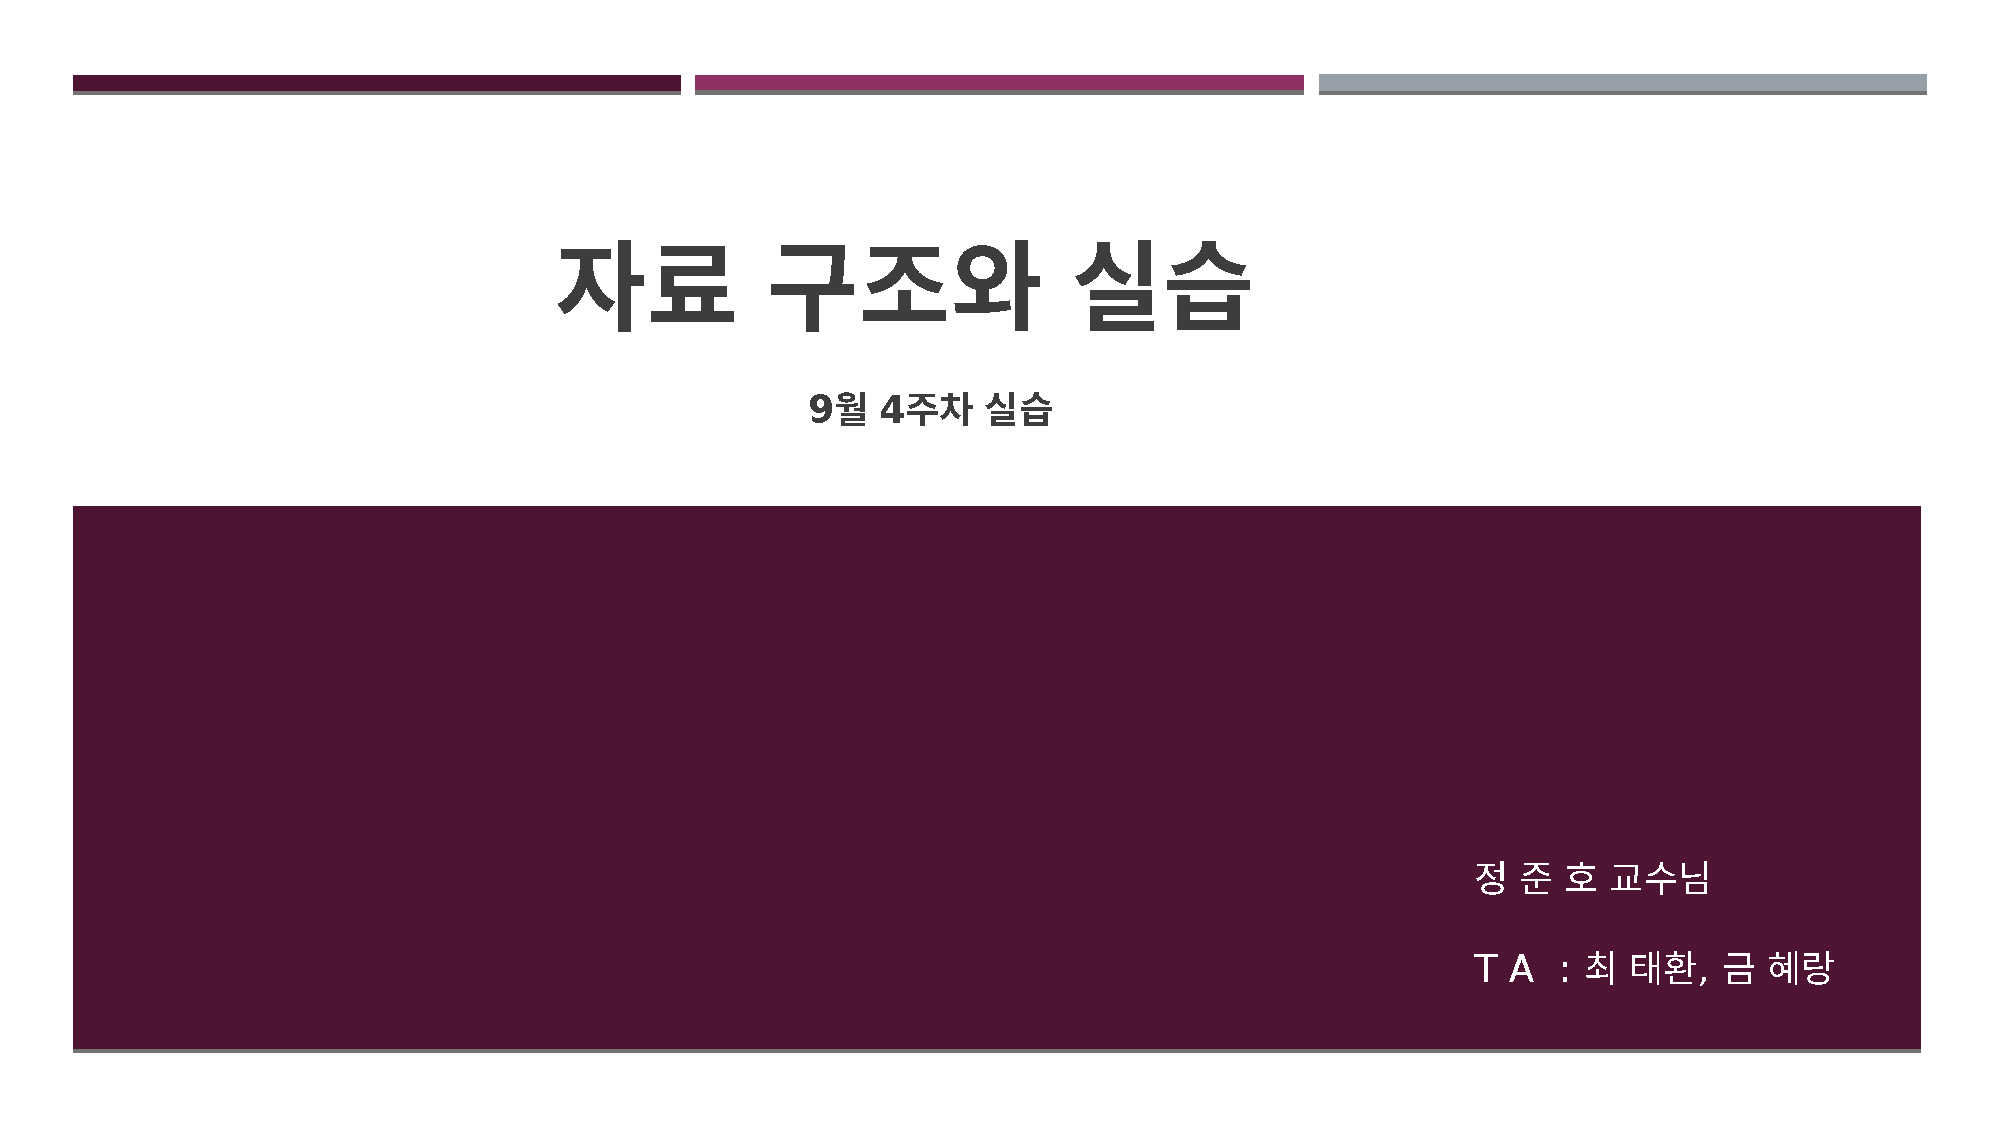
\includegraphics[width=\textwidth]{1.png}	


\section*{2.}	
\lstinputlisting{2.c}	
\includegraphics[width=\textwidth]{2.png}	


\section*{3.}
\lstinputlisting{3.c}	
\includegraphics[width=\textwidth]{3.png}	


\section*{4.}
\lstinputlisting{4.c}	
\includegraphics[width=\textwidth]{4.png}	


\includegraphics[page=3, width=\textwidth]{1.pdf}
%\section*{5.}
\lstinputlisting{5.c}	
\includegraphics[width=\textwidth]{5.png}	


\includegraphics[page=4, width=\textwidth]{1.pdf}
%\section*{6.}
\lstinputlisting{6.c}	
\includegraphics[width=\textwidth]{6.png}	


\includegraphics[page=5, scale=0.7, trim=3cm 2cm 5cm 3cm, clip]{1.pdf}
%\section*{7.}
\lstinputlisting{7.c}	
\includegraphics[width=\textwidth]{7.png}	


\includegraphics[page=6, scale=0.7, trim=3cm 4cm 1cm 3cm, clip]{1.pdf}
\lstinputlisting{8.c}	
\includegraphics[width=\textwidth]{8.png}	
%\section*{8.}
\end{document}
